% Options for packages loaded elsewhere
\PassOptionsToPackage{unicode}{hyperref}
\PassOptionsToPackage{hyphens}{url}
%
\documentclass[
]{article}
\usepackage{amsmath,amssymb}
\usepackage{lmodern}
\usepackage{iftex}
\ifPDFTeX
  \usepackage[T1]{fontenc}
  \usepackage[utf8]{inputenc}
  \usepackage{textcomp} % provide euro and other symbols
\else % if luatex or xetex
  \usepackage{unicode-math}
  \defaultfontfeatures{Scale=MatchLowercase}
  \defaultfontfeatures[\rmfamily]{Ligatures=TeX,Scale=1}
\fi
% Use upquote if available, for straight quotes in verbatim environments
\IfFileExists{upquote.sty}{\usepackage{upquote}}{}
\IfFileExists{microtype.sty}{% use microtype if available
  \usepackage[]{microtype}
  \UseMicrotypeSet[protrusion]{basicmath} % disable protrusion for tt fonts
}{}
\makeatletter
\@ifundefined{KOMAClassName}{% if non-KOMA class
  \IfFileExists{parskip.sty}{%
    \usepackage{parskip}
  }{% else
    \setlength{\parindent}{0pt}
    \setlength{\parskip}{6pt plus 2pt minus 1pt}}
}{% if KOMA class
  \KOMAoptions{parskip=half}}
\makeatother
\usepackage{xcolor}
\usepackage[margin=1in]{geometry}
\usepackage{graphicx}
\makeatletter
\def\maxwidth{\ifdim\Gin@nat@width>\linewidth\linewidth\else\Gin@nat@width\fi}
\def\maxheight{\ifdim\Gin@nat@height>\textheight\textheight\else\Gin@nat@height\fi}
\makeatother
% Scale images if necessary, so that they will not overflow the page
% margins by default, and it is still possible to overwrite the defaults
% using explicit options in \includegraphics[width, height, ...]{}
\setkeys{Gin}{width=\maxwidth,height=\maxheight,keepaspectratio}
% Set default figure placement to htbp
\makeatletter
\def\fps@figure{htbp}
\makeatother
\setlength{\emergencystretch}{3em} % prevent overfull lines
\providecommand{\tightlist}{%
  \setlength{\itemsep}{0pt}\setlength{\parskip}{0pt}}
\setcounter{secnumdepth}{-\maxdimen} % remove section numbering
\ifLuaTeX
  \usepackage{selnolig}  % disable illegal ligatures
\fi
\IfFileExists{bookmark.sty}{\usepackage{bookmark}}{\usepackage{hyperref}}
\IfFileExists{xurl.sty}{\usepackage{xurl}}{} % add URL line breaks if available
\urlstyle{same} % disable monospaced font for URLs
\hypersetup{
  pdftitle={The penguins of Antarctica},
  pdfauthor={Selina Baldauf},
  hidelinks,
  pdfcreator={LaTeX via pandoc}}

\title{The penguins of Antarctica}
\author{Selina Baldauf}
\date{25/3/2022}

\begin{document}
\maketitle

\hypertarget{introduction}{%
\section{Introduction}\label{introduction}}

There are three main penguin species in Antarctica (\emph{Chinstrap},
\emph{Gentoo}, \emph{Adelie}). You can see them in the following figure:

\begin{figure}
\centering
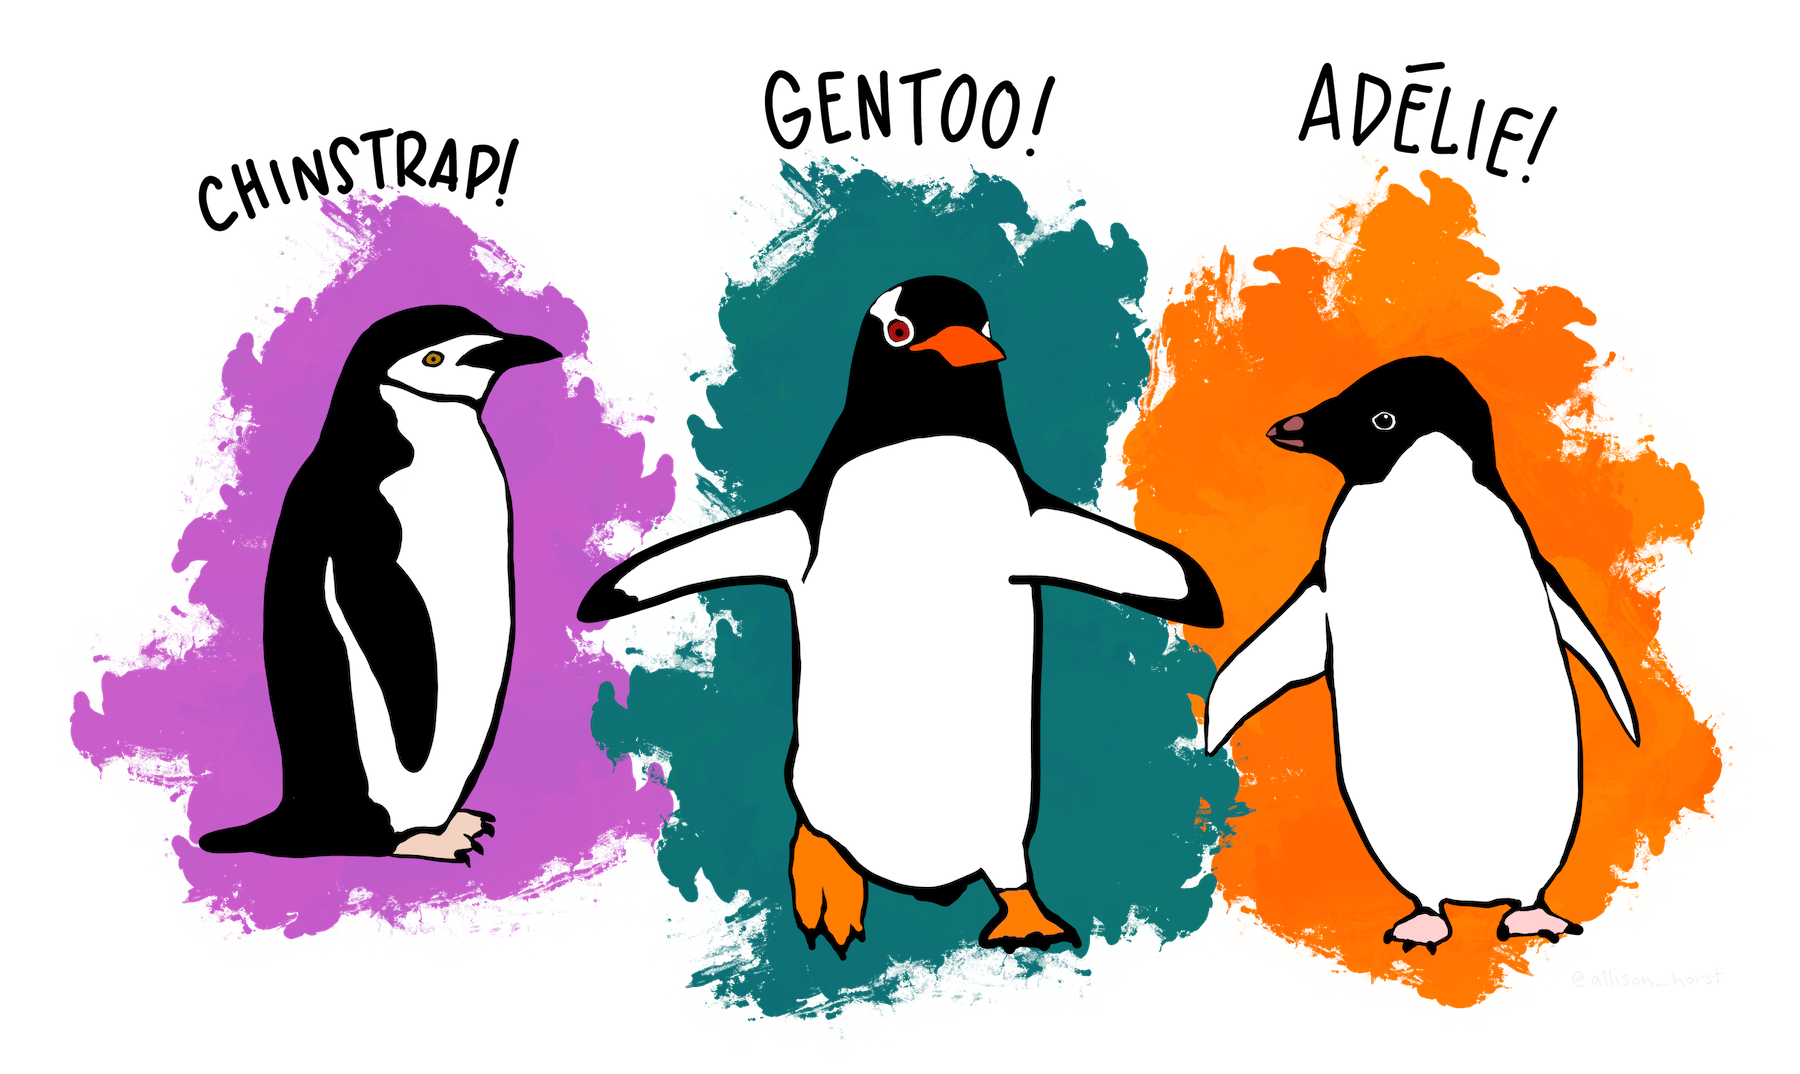
\includegraphics{https://raw.githubusercontent.com/allisonhorst/palmerpenguins/main/man/figures/lter_penguins.png}
\caption{Artwork by \href{https://twitter.com/allison_horst}{Allison
Horst}}
\end{figure}

In this paper we want to answer the following questions

\begin{enumerate}
\def\labelenumi{\arabic{enumi}.}
\tightlist
\item
  How bill depth depends on bill length?
\item
  Which penguin species has the highest body mass?
\end{enumerate}

\hypertarget{methods}{%
\section{Methods}\label{methods}}

\hypertarget{the-data}{%
\subsection{The data}\label{the-data}}

The data was collected on islands in Antarctica and published by Gorman
et al.~(2014). You can find the original paper with the title
``Ecological sexual dimorphism and environmental variability within a
community of Antarctic penguins (genus \emph{Pygoscelis})'' in PLoS
ONE\footnote{paper available
  \href{https://doi.org/10.1371/journal.pone.0090081}{here}.}

The data is published via the \texttt{palmerpenguins} R package which
you can find \href{https://allisonhorst.github.io/palmerpenguins/}{on
this website}.

\textbf{The data contains (among others) the following measurements:}

\begin{itemize}
\tightlist
\item
  bill length
\item
  bill depth
\item
  body mass
\item
  sex

  \begin{itemize}
  \tightlist
  \item
    male
  \item
    female
  \end{itemize}
\end{itemize}

\hypertarget{the-analysis}{%
\subsection{The analysis}\label{the-analysis}}

We did some plots, calculated some summary statistics and a linear model
of the form \(y = ax + b\)

\hypertarget{results}{%
\section{Results}\label{results}}

Will be added later

\end{document}
